\batchmode
\documentclass[a4paper,oneside,article]{memoir}

\usepackage[utf8]{inputenc}
\usepackage[final,hyperindex,hyperfootnotes]{hyperref}
\usepackage{graphicx}

\title{Introduction to Fiji (ImageJ)}
\author{Graeme Ball and Dominic Waithe}
\date{}

\begin{document}
  \maketitle

  \chapter{Basic Image Characteristics}

    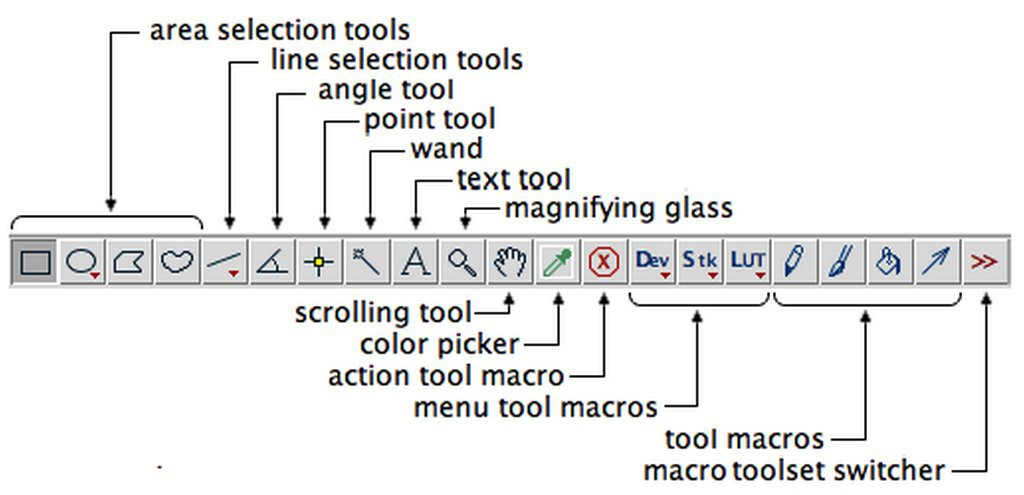
\includegraphics[width=\textwidth]{ImageJ-toolbar.jpeg}

    \begin{enumerate}[(a)]
      \item Start by opening the Fiji application which you should have
      previously downloaded. This is achieved by either double-clicking
      the Fiji.app (mac) file or the ``Fiji Image Win64'' file in the
      directory where you saved the files.

      \item Now we want to open an image. Before starting this course
      you should have downloaded and unzipped some image files. Goto
      this directory and drag the image named ``Cell\_Colony.tif'' onto
      the Fiji toolbar (to the area just below the icons). The image
      should then open. If this fails you can open the image using the
      Fiji menu system. Goto File, then Open. (File$\rightarrow$Open).
      From here find and open the images you downloaded before this
      practical.

      \item Try zooming in on the Cell Colony image (Magnifying glass
      tool button + mouse, or the +/- keys). Do you notice anything odd
      or unnatural about the background? hint: this file was once a
      jpeg. Always keep your raw data and do not use image compression.
      \emph{Don't rely on compression formats for long-term storage.}

      Invert the Cell Colony image (Edit$\rightarrow$Invert).
      Imagine for a moment that the distorted background is noise: now
      find one of the faint ``particles'' (actually a colony), and draw
      a line through it that is around 5-10x as long as the ``particle''
      is wide. The line tool is the fifth one along the toolbar. You can
      plot a line profile using Analyze$\rightarrow$Plot Profile (Ctrl-K
      (PC) and Cmd-K(mac)). Get a feel for what the intensity of the
      ``signal'' is compared to the random intensity variations in the
      background?

      \item Now take your inverted Cell Colony image and duplicate it
      two times (Image$\rightarrow$Duplicate or Ctrl-Shift-D(PC) ,
      Cmd-Shift-D(mac)). Try multiplying one of the duplicate images
      by 8, and try dividing the other by 8 (use
      Process$\rightarrow$Math$\rightarrow$Multiply\dots{} and
      Divide\dots{}). Place the mouse cursor over the pixels in the
      results. On the toolbar you will see the pixel intensities. Do you
      notice anything strange about the numbers?Can you see why it is
      important to appropriate image exposure and/or gain settings?

      Note that Image$\rightarrow$Adjust$\rightarrow$Brightness/Contrast
      (Ctrl-Shift-C (PC), Cmd-Shift-C(mac)) cannot undo the damage of
      exceeding or not utilising your detector's dynamic range. Ideally
      you want to just about fill the range available --- no more, no
      less. To visualise whether there is saturation or clipping of the
      image intensities, change the Look-Up-Table of the image. If you
      choose the HiLo LUT you can view saturation as red pixels in the
      image and clipping of low intensities as blue pixels.
      Image$\rightarrow$Look Up Tables $\rightarrow$ HiLo. Now
      experiment with the Brightness/Contrast settings as before and
      see what happens.
    \end{enumerate}

  \chapter{Thresholding and binary operations}
    \label{sec:threshold}

    \begin{enumerate}[(a)]
      \item The image histogram is an important concept to understand.
      Open the image cell\_fluorescent.tif. Select the whole image,
      Edit$\rightarrow$Selection$\rightarrow$Select All (Ctrl-A (PC),
      Cmd-A(mac)). Analyze$\rightarrow$Histogram. The plot displays
      the number of pixels in each intensity bin (256 bins is the
      default). If you click the list button you can examine the raw
      numbers. Notice the statistics displayed underneath, including
      minimum and maximum values, standard deviation, mean etc.

      Select a dim region (1) of the image using the Oval selection
      tool and repeat the analysis. Now select a region entirely within
      the cell body (2) and look at the histogram. Finally, examine the
      histogram for a region that is half cell body, half dim region (3).
      Can you explain what you see? This can be used as the basis for
      distinguishing the two regions, using a thresholding method

      \item Display settings allow the displayed values to be changed
      without altering the underlying pixel values in the raw data
      --- some sort of transfer function maps raw to displayed values.
      Open the blobs.tif sample Image.
      Image$\rightarrow$Adjust$\rightarrow$Brightness/Contrast is the
      normal way to adjust display settings. There are buttons to
      Auto-adjust and Reset to the original settings. The Set button
      allows you to type in values manually, and even propagate the
      settings to other channels and images. For example, try setting
      the minimum and maximum values to 127 and 196, and reset to the
      original settings. You should be careful with the final button,
      Apply. Set min/max to 127/196 again, but this time click Apply.
      You should find that Reset no longer works. Try
      File$\rightarrow$Save As$\rightarrow$Text Image and see if you
      can understand what has happened.

      You may have used a gamma correction function in other image
      analysis packages --- this maps the raw intensity data to
      displayed intensities in a non-linear way, emphasizing dim or
      bright features by assigning more levels to them. ImageJ does
      have a gamma correction function, but it is hidden in under
      Process$\rightarrow$Math$\rightarrow$Gamma. Note that this is a
      transform rather than a reversible mapping! If you click the
      Preview button you can see the effect of changing Gamma from a
      low value (emphasizing dim features) to a high value (emphasizing
      bright features). Use this only for illustration however.
      Non-linear mappings must be avoided for analysis because they
      distort relationships in data.

      \item \label{itm:automatic-threshold}
      Segmentation is a means of separating image pixels into
      different subsets. The most common method to segment an image,
      is to apply a threshold. Open the cell\_fluorescent.tif sample
      image. Convert the image to single 8-bit channel by clicking
      Image$\rightarrow$Type$\rightarrow$8-bit.We only want to apply
      a threshold in one-colour channel to simplify the thresholding.
      Now we want to duplicate this image so we can experiment with
      different algorithms Image$\rightarrow$Duplicate.  Next open
      the threshold dialog Image$\rightarrow$Adjust$\rightarrow$Threshold.
      Move the threshold slide-bars under the histogram and notice
      the effect. Try and find a level with segments the blobs from
      their background and click apply. You have now segmented an image.

      \item Go back to the 8-bit version of the image and duplicate
      a fresh copy. Now once again goto the threshold dialog
      Image$\rightarrow$Adjust$\rightarrow$Threshold. This time rather
      than manually changing the slider, click on the box which says
      Default and then click `Otsu'. This is an automatic thresholding
      algorithm which attempts to find a threshold value which best
      segments the image population in the intensity histogram. Click
      apply to see the output binary image. Algorithms such as `Otsu'
      can be used to automatically segment images without human
      interaction.

      \item Go back to the 8-bit version of the image and duplicate
      another fresh copy. Add some noise
      Process$\rightarrow$Noise$\rightarrow$RandomJ$\rightarrow$Poisson.
      Poisson is the most common noise found in microscopy. Apply a
      Mean 10.0 to the image. Next once again apply a threshold and
      use the 'Otsu' algorithm. What you do you notice? Try this again
      but using mean noise of 20 and 60. What do you notice as the
      noise gets worse? How do think having noisy data might affect
      your analysis?

      \item Go back to the 8-bit cell\_fluorescent.tif image. Goto the
      threshold dialog  Image$\rightarrow$Adjust$\rightarrow$Threshold.
      Choose an arbitrary threshold. Now we are going to manipulate the
      resultant binary image using binary morphological operations.
      Goto Process$\rightarrow$Binary and click erode. What do you
      notice? Goto Edit$\rightarrow$Invert and then click
      Process$\rightarrow$Binary$\rightarrow$erode once again. What do
      you notice? Create a fresh binary image. Try some of the other
      options. Invert the image and see how the operation changes its
      effect.
    \end{enumerate}

  \chapter{More about image display}
    \begin{enumerate}[(a)]
      \item Multi-channel images differ from an RGB image in that each
      channel is a completely separate image. Fiji has a number of
      tools to manipulate channels, their display, and conversion to
      and from RGB images.

      Take a look at the Leaf.tif sample image, this time opening
      Image$\rightarrow$Color$\rightarrow$Channels Tool. Click 'Yes' to
      the dialog. In addition to the usual ``c'' slider under the image
      you now have a tick box for each channel that can be used to
      select a channel. You also have a choice box at the top used to
      set the viewing mode, and a More \textgreater{}\textgreater{}
      choice box at the bottom. Look at the options in the
      More \textgreater{}\textgreater{} menu, and try changing the
      colour of the channel you are looking at (the Merge and
      Split Channels and Convert to RGB options are the same as those
      in the Color menu). Note that the choice of colour is up to you
      and not dependent on the wavelength of the channel for instance.
      Often grayscale is the best choice for analysis, and remember
      that the human eye is sensitive to
      Green\textgreater{}Red\textgreater{}Blue in that order.

      Now try changing the Color view mode to Composite. You should see
      all channels, and have the option of turning each one on/off. If
      you move the channel slider now, notice that the colour of the
      window border and info string at the top left change to match the
      channel you have selected. Now try changing to the second channel
      (``green'') and adjusting brightness/contrast (Ctrl-Shift-C(PC),
      Cmd-Shift-C(mac)) and you should see that the histogram is also
      coloured to reflect the channel colour you have set. Try Convert
      to RGB on your composite view. Notice that the R,G,B values you
      see when you mouseover the image are difficult to interpret.

      In general, it is good practice to preserve separate channels for
      processing and analysis until the final stages of producing a figure.

      \item Look-Up Tables (LUTs) map intensity values to a displayed
      colour. Open the Blobs.tif image. Goto
      Image$\rightarrow$Lookup Tables$\rightarrow$Invert LUT. What values
      do you see when you mouseover the dark and bright regions of the
      image? Is this what you expected? Have a look at
      Image$\rightarrow$Color$\rightarrow$Show LUT and/or
      Image$\rightarrow$Color$\rightarrow$Edit LUT and you should be able
      to see what is going on.

      The LUT for an image can be changed using
      Image$\rightarrow$Lookup Tables - try Grays. Now that you have the
      default LUT you should find the intensities values in the image
      make more sense. Try some of the more colourful schemes: Fire,
      Rainbow RGB etc. and examine how the colour changes with intensity
      using Show LUT and/or Edit LUT. They can be helpful for making
      small changes in intensity obvious, and extremely useful for
      visualizing measurements such as FRET efficiency or fluorescence
      lifetime. Using Edit LUT try making your own LUT that shows Blob
      centre, boundary and background in different colours.
    \end{enumerate}

  \chapter{Colocalisation}
    \begin{enumerate}[(a)]
      \item Open the image neuron.tif. We only want to work with the
      first and last channel. One way to separate them from the
      original image is to use image$\rightarrow$Duplicate. Check the
      box marked `Duplicate HyperStack' but type `1' in the channels
      box rather than having `1--4'. Click `ok'. Repeat, but duplicate
      channel 4 instead. You should now have two stacks. In both cases
      goto Image$\rightarrow$Type$\rightarrow$8-bit. This is a good
      habit to do before colocalisation as colour info can sometimes
      disrupt the algorithm. Now pick a stack z-slice, duplicate this
      slice only and repeat for the same z-slice in the other stack.
      In one of the z-stacks change the z-slice by at least 5 levels
      and then duplicate this slice. This second image is a good
      comparison for this practical: it is similar but should be
      different enough not to correlate with the first.

      \item Goto Analyze$\rightarrow$Colocalisation$\rightarrow$ Coloc 2
      function. Click the first two slices that you created, one from
      either channel, leave the `ROI mask' unselected for now. Run the
      colocalisation with all the parameters checked. Look for the
      output marked Pearson's R value (no threshold). What value do
      you get? Try this again for the control slice. Is the control
      value strangely high? This is what happens when your images
      contain large areas of background such as these. Even zero pixels
      will have an effect.

      \item This time repeat the exercise but with an oval selection
      surrounding only the fluorescent region of the cell with no
      minimal background. Next goto
      Edit$\rightarrow$Selection$\rightarrow$Create Mask.  In the
      `Coloc 2' dialog box you will have to select under `mask or ROI'
      the newly created mask image entitled `Mask'. Run the `Coloc 2'
      plugin. What do you notice about the Pearson's R-value now? What
      is the effect of removing the background pixels on the R-value
      of the test and control condition? This represents a more focused
      use of the Pearson’s test.

      \item Repeat the previous step but this time create a mask from
      one of the channels using the thresholding technique described in
      \Sref{sec:threshold}.\ref{itm:automatic-threshold}. You may have
      to invert the threshold mask for it to work correctly
      Image$\rightarrow$Invert. To establish what areas are being
      included in the colocalisation analysis make sure the `Display
      Images in Results' checkbox is positive. When you run the plugin
      you can view the included pixels by selecting either `Channel 1'
      or `Channel 2' from the drop-down box at the top of the output dialog.

      \item Does the colocalisation R-value change if you change the
      mask? By choosing threshold values which are harsher and more
      restrictive you will create a smaller mask area. Try this and see
      how the R-value changes during the colocalisation analysis. This
      exercise should show why it is important to be consistent when
      applying masking in colocalisation data.
    \end{enumerate}

\end{document}
